% !TEX root = main_org.tex

\chapter{Toy MC simulation}

\subsection{Toy Monte Calro simulation}
In this appendix, we will the Monte Carlo simulation to check the correlation between two different flow harmonics and check the systematics response to $Q$-Cumulant method(QC) and Scalar Product method(SP). 

\smallskip	
	
	Since, $SC(m,n)$ is defined as like $$ \langle v_n^2 v_m^2 \rangle - \langle v_n^2 \rangle \langle v_m^2 \rangle $$
	it is not easy to calculate directly $SC(m,n)$ from arbitary $v_n$ and $v_m$ which fluctuate event by event. So, in this Toy Monte Calro simulation, we consider simplest case. i.e the uniform flow distribution.
	The uniform flow distribution is defined as like
	
	\begin{equation}
		f(v_n) = const, \hskip5mm v_{min} < v_n < v_{max}
	\end{equation}
	
	In this configuration, we can easily assume that the function of flow $v_n$ can be normalized with
	
	\begin{eqnarray}
		1 &=& \int_{-\infty}^{\infty}f(v_n)dv \\
			&=& \int_{v_{min}}^{v_{max}}const ~ dv \\
			&=& cont (v_{max} - v_{min} )
	\end{eqnarray}
	
	
	so,
	\begin{equation}
		const = \frac{1}{v_{max} - v_{min} }
	\end{equation}
	\smallskip
	
	Then the final normalized unifrom flow distribution is
	\begin{equation}
		f(v_n) = \frac{1}{v_{max} - v_{min}}
	\end{equation}
	\smallskip
	
	And if we assume the mean value of given order flow harmonics as $\mu_v$, then it follows
		
		
	\begin{eqnarray}
		1 &=& \int_{-\infty}^{\infty}vf(v)dv \\
			&=& \int_{v_{min}}^{v_{max}} v \frac{1}{v_{max} - v_{min}}  dv \\
			&=& \frac{1}{v_{max} - v_{min}} \frac{v_{max}^2 - v_{min}^2}{2}
	\end{eqnarray}

	and finally we have 
	
	\begin{equation}
		\mu_v = \frac{v_{max} - v_{min}}{2}
	\end{equation}
	\smallskip
	
	To calculated standard deviation($\sigma_v$) for event fluctuations, use the definiation of expectaion value of a random variables.
	
	\begin{equation}
		\mu_x = E[x] = \int_{-\infty}^{\infty}{xf(x)dx}
	\end{equation}
	\begin{equation}
		\sigma_x^2 = V[x] = E[(x-E[x])^2] = \int_{-\infty}^{\infty}{(x-\mu_x)^2 f(x) dx}
	\end{equation}
	\smallskip
	
	So, we can get straightforwardly
	
	\begin{equation}
		\sigma_v^2 = \frac{1}{12}(v_{max} - v_{min})^2
	\end{equation}
	
	or,
	
	\begin{equation}
		\sigma_v = \frac{1}{2\sqrt{3}}(v_{max} - v_{min})
	\end{equation}
	\smallskip
	
	
	So, for the uniform distribution Toy models, we can express the flow $v_n$ and its fluctuation with events($\sigma_v$) as term as uniform flow distribution ($v_{max}$ and $v_{min}$)
	
	\begin{equation}
		\langle v \rangle = \frac{v_{max} + v_{min}}{2}
	\end{equation}
	\begin{equation}
		\langle v^2 \rangle = \frac{v_{max}^2 + v_{max}v_{min} + v_{min}^2}{3}
	\end{equation}
	\begin{equation}
		\langle v^3 \rangle = \frac{1}{4} (v_{max} + v_{min})(v_{max}^2 + v_{min}^2 )
	\end{equation}	
	\begin{equation}
		\langle v^4 \rangle = \frac{1}{5}(v_{max}^4 + v_{max}^3v_{min} + v_{max}^2v_{min}^2 + v_{max}v_{min}^3 + v_{min}^4)
	\end{equation}
	\smallskip
	
	With above equations, we now can express the $SC(m,n)$ as term of $v_{max}$ and $v_{min}$ only. For example, if we set $v_2$ and $v_3$ to have uniform distribution such as
	
	\begin{itemize}
	\item $v_2$ = Uniform[0.05, 0.08]
	\item $v_3 = 0.1 - v_2$
	\end{itemize}
	
	then the $SC(3,2)$ will be express as like 
	\begin{eqnarray}
		SC(3,2) &=& \langle v_3^2 v_2^2 \rangle - \langle v_3^2 \rangle \langle v_2^2 \rangle \\
		&=& \langle x^2 (0.1-x)^2 \rangle - \langle x^2 \rangle \langle (0.1-x)^2 \rangle \\
		&=& \langle x^2(0.01 - 0.2x + x^2 ) \rangle - \langle x^2 \rangle \langle (0.01 - 0.2x + x^2 ) \rangle \\
		&=& \langle 0.01x^2 \rangle - \langle 0.2x^3 \rangle + \langle x^4 \rangle - \langle x^2 \rangle ( 0.01 - \langle 0.2 x \rangle + \langle x^2 \rangle ) \\
		&=& - (0.2)\langle x^3 \rangle + \langle x^4 \rangle + 0.2 \langle x \rangle \langle x^2 \rangle - \langle x^2 \rangle^2 \\
		&=& -(0.2) \frac{1}{4}(v_{max}+v_{min})(v_{max}^2 + v_{min}^2) \nonumber \\
		&& +\frac{1}{5}(v_{max}^4 + v_{max}^3v_{min} + v_{max}^2v_{min}^2 + v_{max}v_{min}^3 + v_{min}^4)  \nonumber\\
		&& 0.2\frac{v_{max}^2 + v_{max}v_{min} + v_{min}^2}{3} \frac{v_{max}+v_{min}}{2} \nonumber \\
		&& - \frac{v_{max}^2 + v_{max}v_{min} + v_{min}^2}{3}\frac{v_{max}^2 + v_{max}v_{min} + v_{min}^2}{3}
	\end{eqnarray}

 As a results $SC(3,2) \simeq -6.78 \times 10^{-7}$, Also $SC(4,2)$ can be obtained by similar calculations.

In this analysis, we tested with ToyMC simulation for $SC(m,n)$ with both uniform fluctuation case (which is simplest case), and 2-Dim Gaussian fluctuation case (which is more realistic case)
\smallskip
For the uniform fluctuation case, we set $v_n$ as like 
\begin{itemize}
	\item $v_2$ = Uniform[0.04, 0.09]
	\item $v_3$ = 0.1 - $v_2$
	\item $v_4$ = $v_2$ - 0.02	
\end{itemize}

These settings are based on the real flow measurements to have $\langle v_2 \rangle \sim 0.065$  which is similar $v_2$ in mid-central collisions, and setting $v_3$ to have negative correlation with similar as what it is measured. Also $v_4$ have been setted to have positive correlation but a little bit higher than what is measured.
	
\begin{figure}[h]
\begin{center}
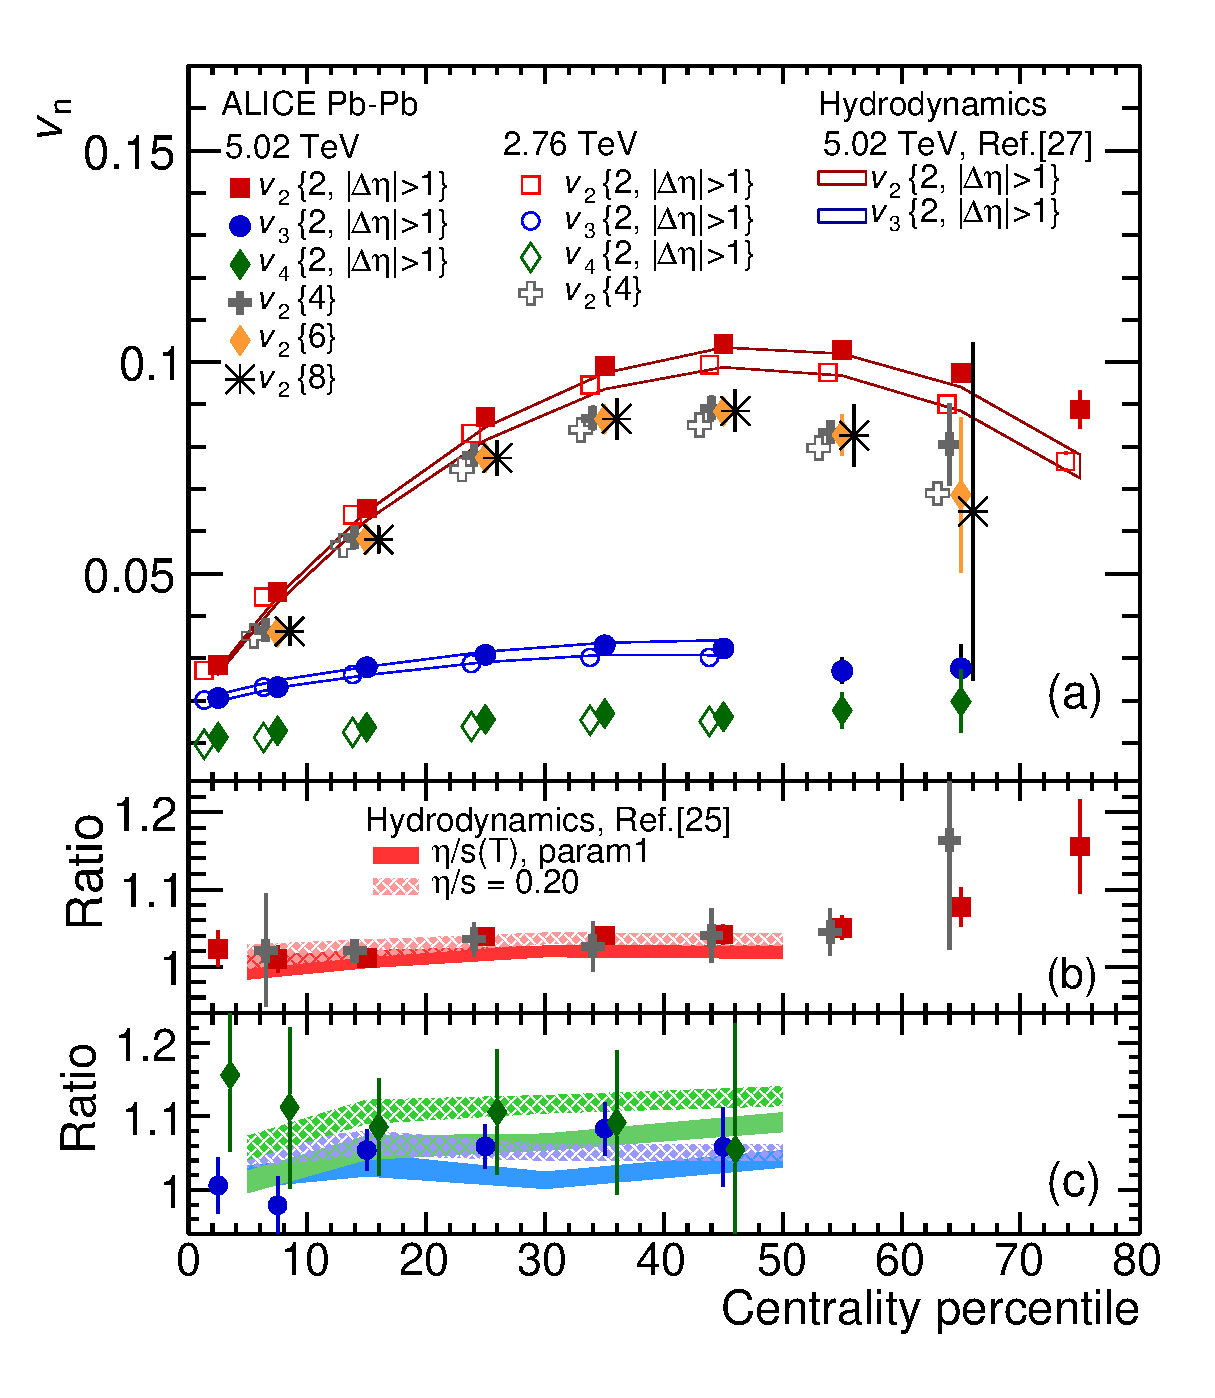
\includegraphics[width=9.0cm]{figures/5tev_vns}
\caption{Flow measurement with ALICE at $\sqrt{S_{NN}} =  2.76$TeV/$c$ and $ 5.02$TeV/$c$ with various measurement methods, also hydrodynamic predictions are drwan as bands}
\label{vn5}
\end{center}
\end{figure}

We performed ToyMC simulations with various multiplicity and run over 1M events per each multiplicity bins. The results are shown in Fig.\ref{fig:ToyMC_Uniform_SC32_woJet} and  \ref{fig:ToyMC_Uniform_SC42_woJet}. As seen in results, both Q-cumulants (QC) and Scalar Product (SP) method were able to capture input value in high multiplicity regions with in $\sim1\%$ errors, but in low multiplicity region, we observe discrepancy between two methods and these effects are most pronounced in lowest multiplicity (corresponding to values for peripheral collisions over 60\% centrality). Neither QC nor SP methods were fully free from these effects. However, because of $\eta$ gap, SP method has disadvantages for the number of combinations(or multiplicity). As the result, QC methods recover better the input value than SP method, and SP method results are always smaller than QC for all multiplicity bins.   
	
\begin{figure}[h]
\centerline{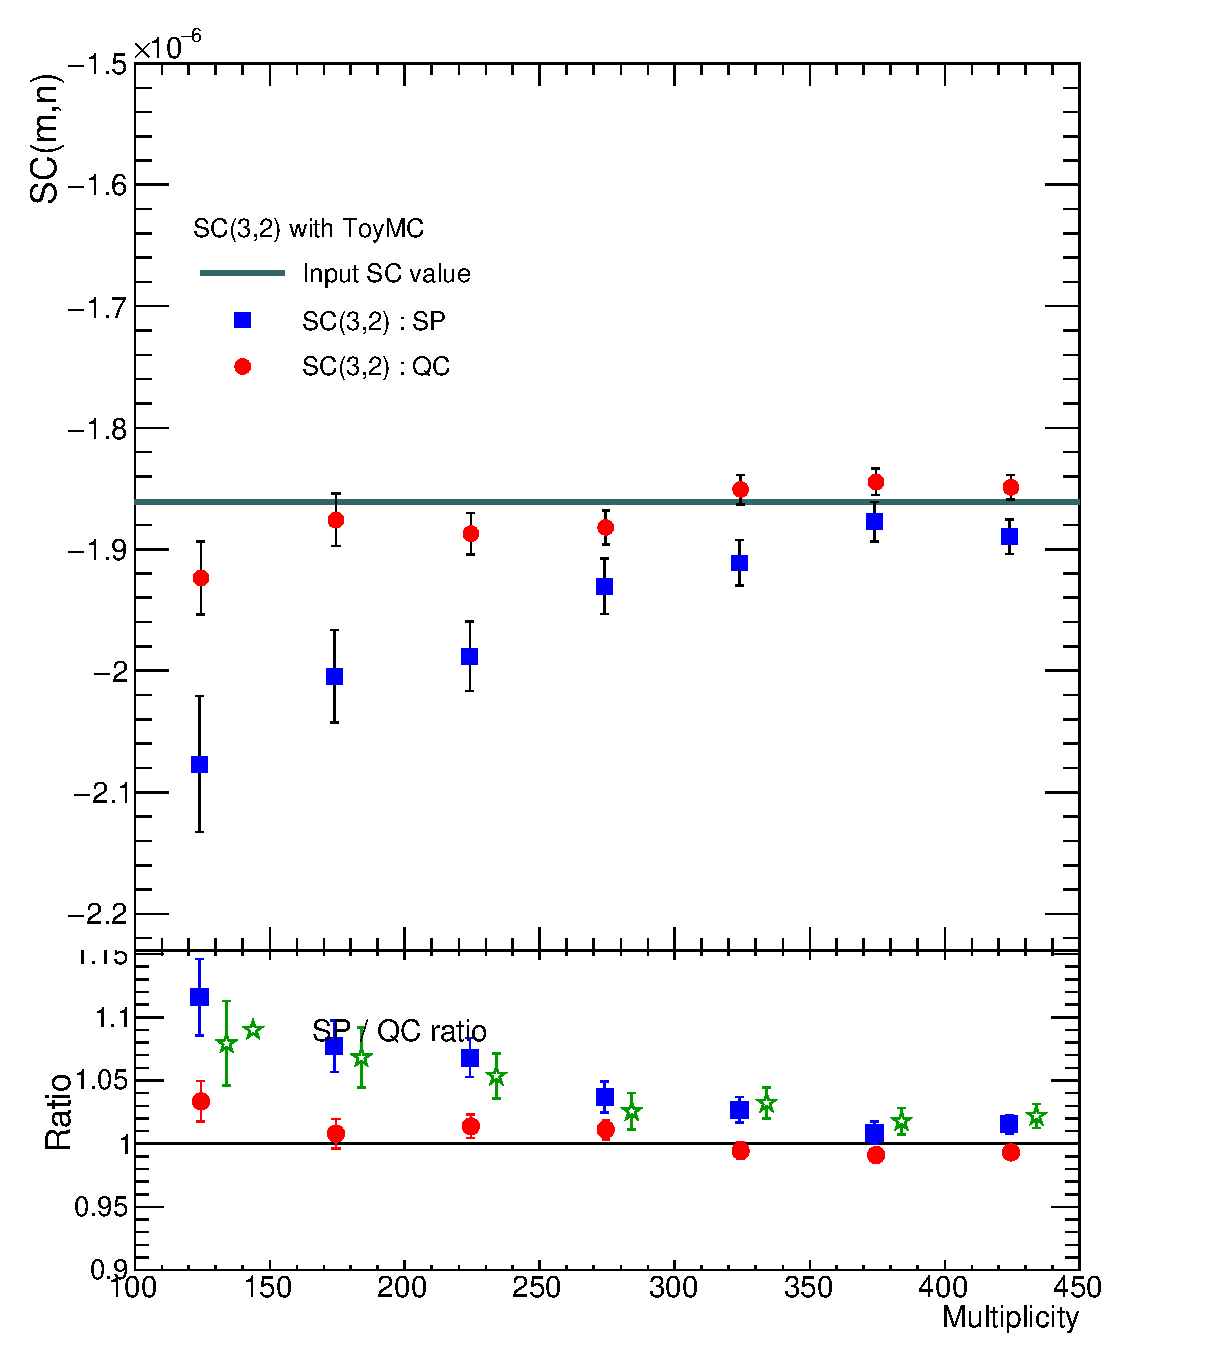
\includegraphics[width=7.0cm]{figures/figs_ToyMC/SC_Comparison_SC32_ToyMC_low_woJet}
\includegraphics[width=7.0cm]{figures/figs_ToyMC/SC_Comparison_SC32_highonly_ToyMC_woJet}}
\caption{Results of ToyMC simulation for SC(3,2) with random uniform distribution of $v_n$ with various multiplicity. The left figure is the result from 50 to 450 multiplicity, and right figure is the result from 500 to 1800 multiplicity. Both Q-cumulatns(QC) and Scalar Product(SP) mehtods are tested and drawn with red and blue color marker. Also ratio to input values are drawn in bottom pad, and the ratio of SP / QC methods are drawn with green marker}
\label{fig:ToyMC_Uniform_SC32_woJet}
\end{figure}


\begin{figure}[h]
\centerline{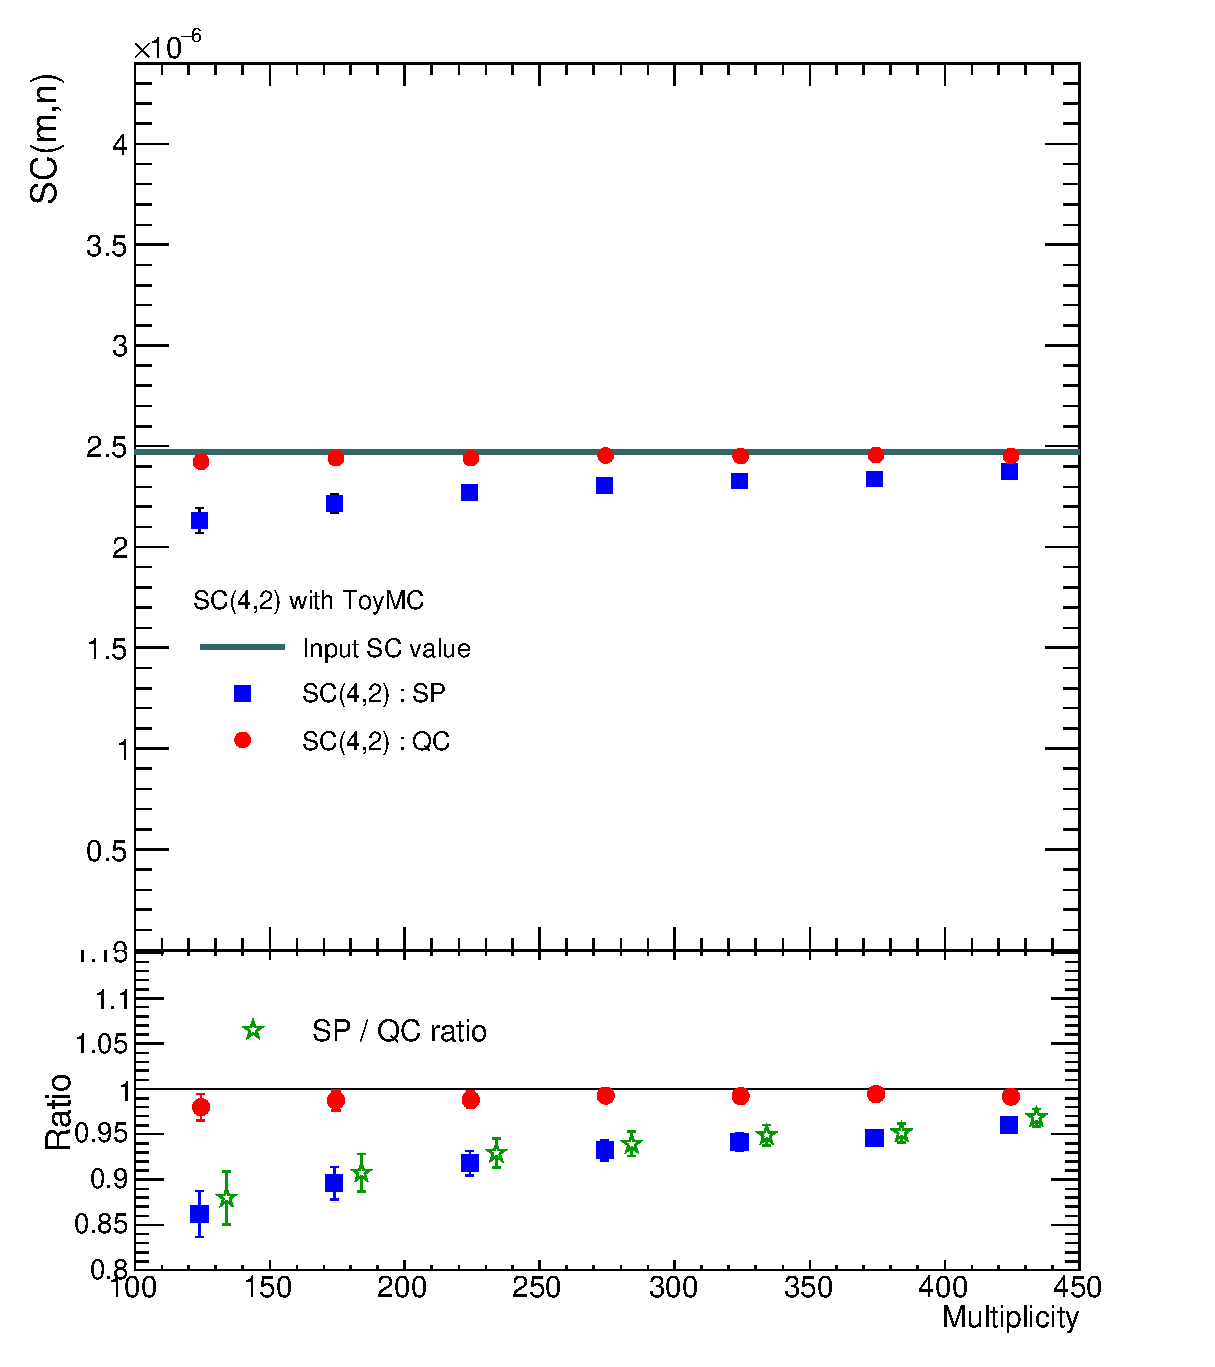
\includegraphics[width=7.0cm]{figures/figs_ToyMC/SC_Comparison_SC42_ToyMC_low_woJet}
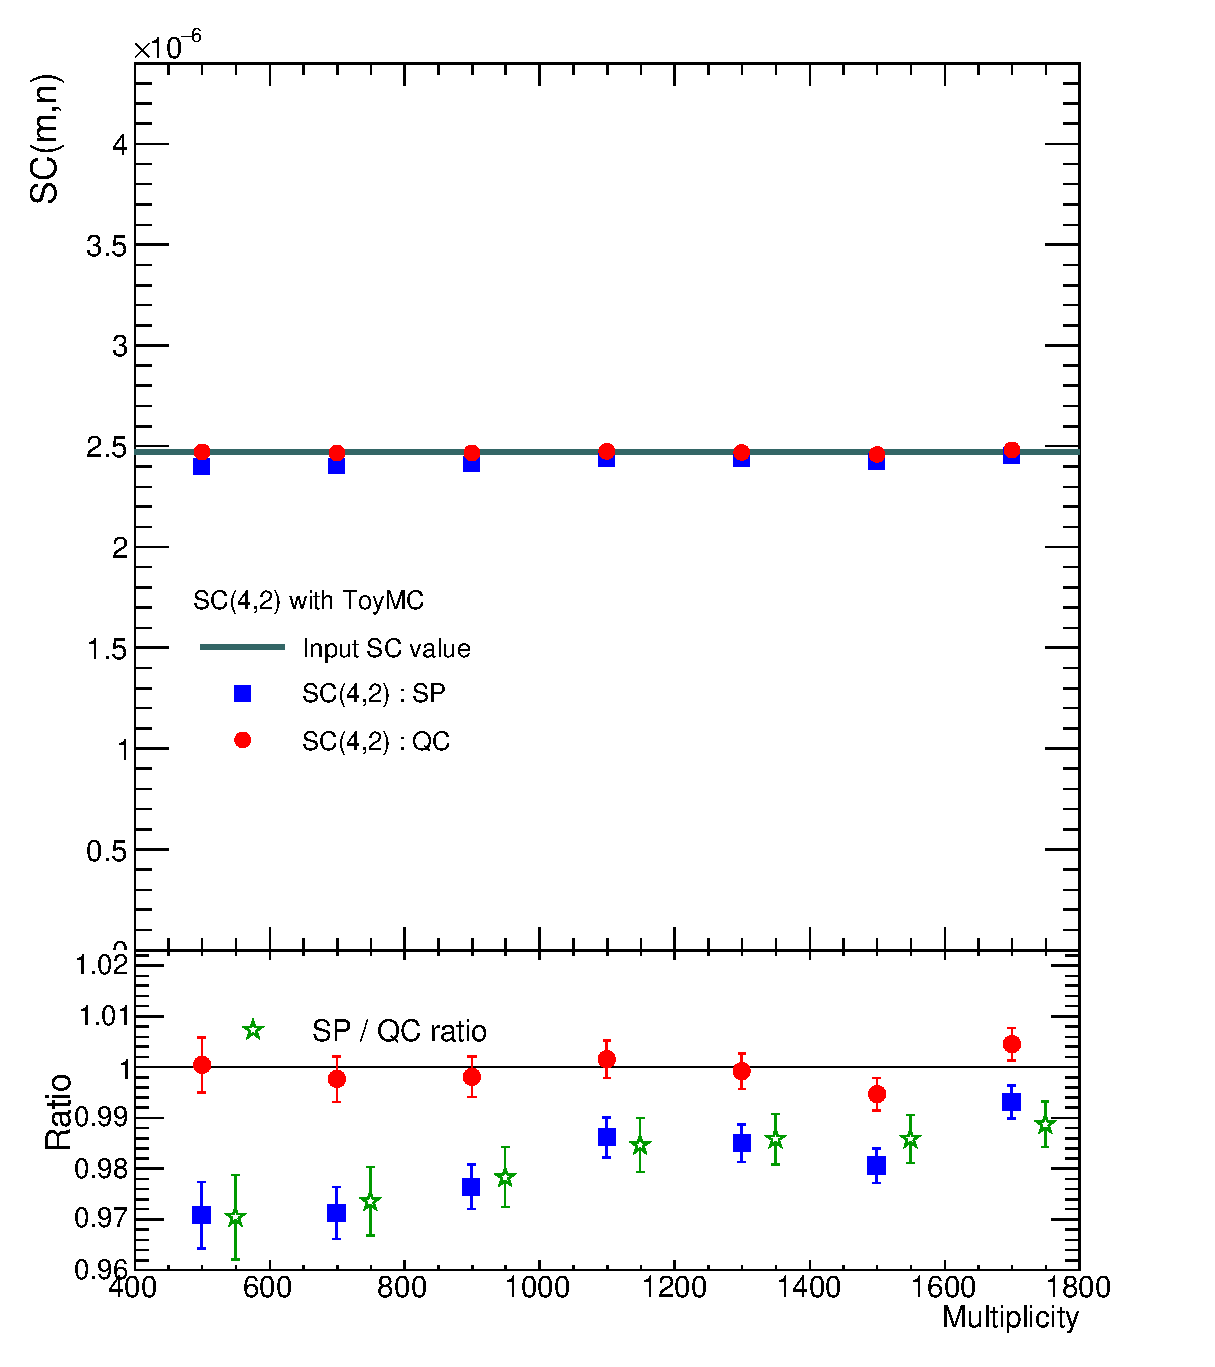
\includegraphics[width=7.0cm]{figures/figs_ToyMC/SC_Comparison_SC42_highonly_ToyMC_woJet}}
\caption{Results of ToyMC simulation for SC(4,2) with random uniform distribution of $v_n$ with various multiplicity. The left figure is the result from 50 to 450 multiplicity, and right figure is the result from 500 to 1800 multiplicity. Both Q-cumulatns(QC) and Scalar Product(SP) mehtods are tested and drawn with red and blue color marker. Also ratio to input values are drawn in bottom pad, and the ratio of SP / QC methods are drawn with green marker}
\label{fig:ToyMC_Uniform_SC42_woJet}
\end{figure}



Also we tested with 2-dim Gaussian like flow fluctuations to try a realistic flow fluctuation taken from a measured distribution.

\begin{equation}
p\left(v_n\right) = \frac{v_n}{\sigma^2}e^{-{\frac{v_n^2}{2\sigma^2}}},
\label{eq:gaussproj1}
\end{equation}

This is the radial projection of a 2 dimensional Gaussian distribution in $\bar v_n$. The $\sigma$ parameter is given by $\sigma=\sqrt{2/\pi}\left<v_n\right>$

then the settings are as like followings
\begin{itemize}
	\item $v_2$ = Bessel Gaussian (mean 0.065)
	\item $v_3$ = 0.04 - ($v_2$/8)
	\item $v_4$ = $v_2 / 6$ 
\end{itemize}

We set $v_n$ to have similar values in real flow values and to have $\sim SC(m,n)$ in mid centralities in ALICE data. The results are shown in Fig.\ref{fig:ToyMC_Gaus}. As same as uniform flow distribution case both method recover input values well and consistent in $1\%$ levels. However when we see the details, we can check that the results from SP methods are always lower than QC methods as like previous results. As the results, the ratio of SP over QC results are above 1 in $SC(3,2)$ case because it' is negative correlation. And ratio of SP over QC are below than 1 in $SC(4,2)$ case. 

\begin{figure}[h]
\centerline{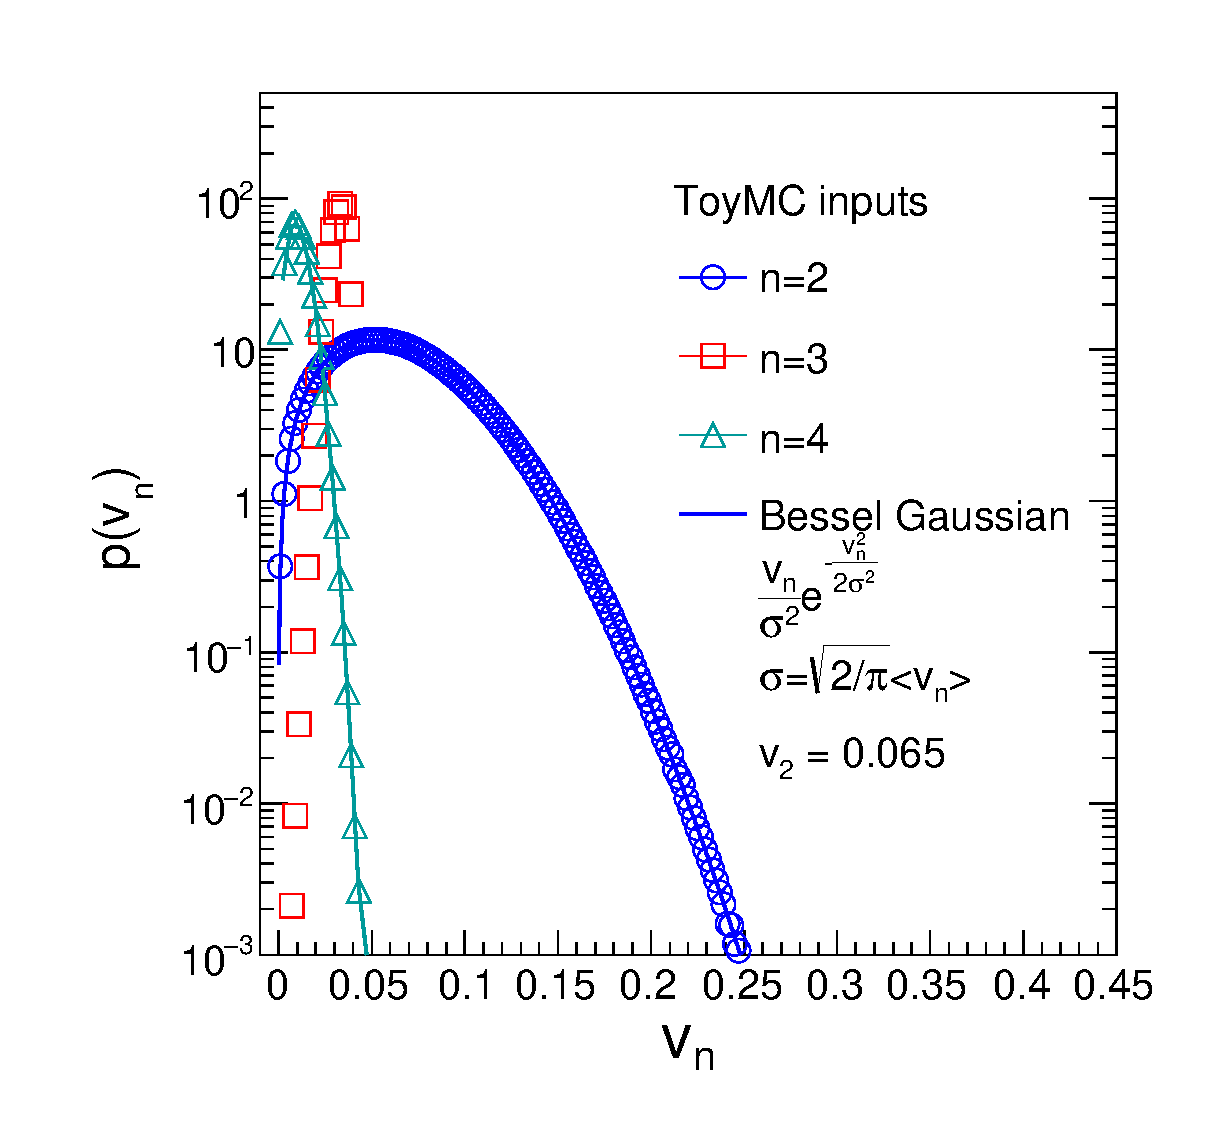
\includegraphics[width=9.0cm]{figures/figs_ToyMC/toymc_vn_input.eps}}
\caption{Event by Event Flow harmoics distributions from Bessel Gaussian function based on \cite{ATLAS:2012jna}}
\label{vn5}
\end{figure}



\begin{figure}[h]
\centerline{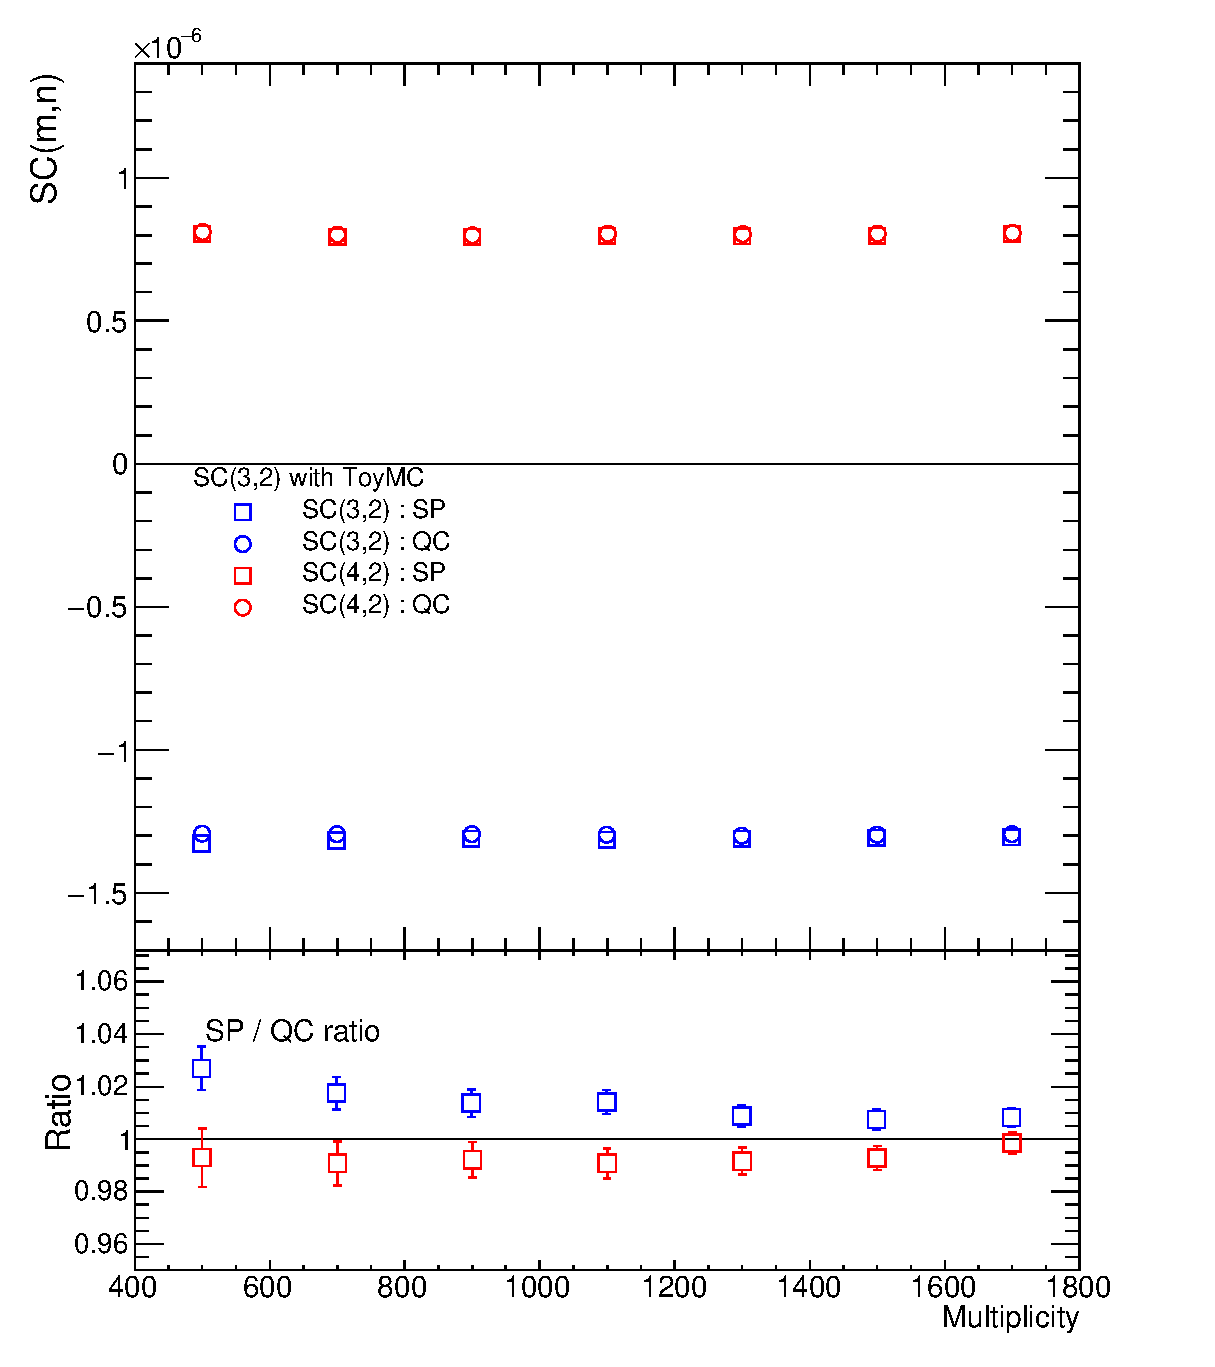
\includegraphics[width=7.0cm]{figures/figs_ToyMC/SC_Comparison_SC_ToyMC_gaus.eps}
}
\caption{Results of ToyMC simulation for SC(m,n) with Bessel Gaussian like distribution, Both SP and QC results were performed and the ratio of two different methods are show in bottom pad}
\label{fig:ToyMC_Gaus}
\end{figure}

\bigskip

\subsection{Test non-flow effects by impose jets from PYTHIA into ToyMC}

$SC(m,n)$ results with HIJING are zero for all centralities for both methods, and also even with the high $p_T$ bins. These suggested that $SC(m,n)$ is not the results from non-flow effects, and it is not sensitive to non-flows. In additional to HIJING results, we now have studied it explicitly with PYTHIA jet particles on $SC(m,n)$. This implies the largest effect from the particles witch stem from jets in PYTHIA in mid central collisions. To check these study, we setup ToyMC as previous section. And use PYHITA8 to impose jet into ToyMC. To see the maximized effects on $SC(m,n)$ we use PYTHIA setting as like followings
\begin{itemize}
	\item $\sqrt{S_{NN}}= 2.76$ TeV 
	\item Phase Space $\hat{p_T} >$  5 GeV/c
	\item Other settings use deafult of PHYTHIA8
\end{itemize}
	and implement jet particles for every events. The $p_T$ spectra and it's ratio to number of  particles in corresponding centralities are drawn in Figure. \ref{fig:ToyMC_PYTHIAjet}. Straitforwadly the jet effects are most pronounced in peripheral collisions and $p_T$ regions more than 1 GeV/c
	
	
\begin{figure}[h]
\centerline{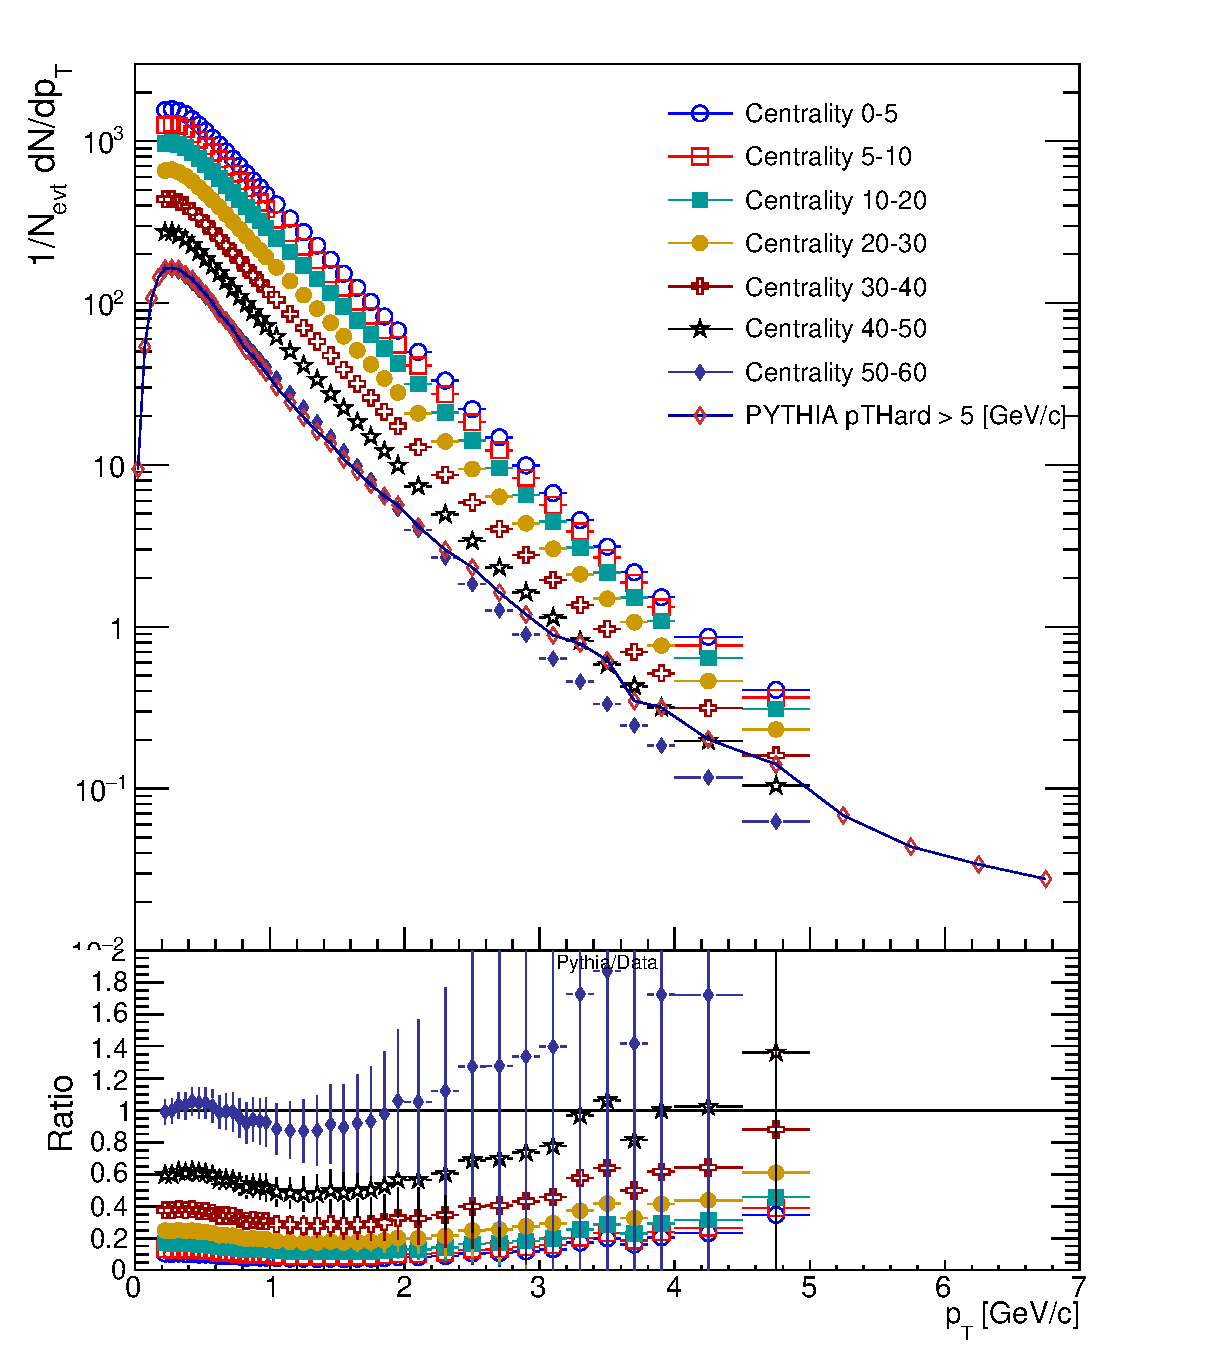
\includegraphics[width=9.0cm]{figures/figs_ToyMC/ptspectra_bulkJet.eps}}
\caption{}
\label{fig:ToyMC_PYTHIAjet}
\end{figure}

	The results of $SC(m,n)$ with ToyMC with jets from PYTHIA is shown in Fig.\ref{fig:ToyMC_withJet}. When we do not implement the PHYTHIA Jet, as we expected, the results of SC(m,n) well capture the input values with around few \% of differences. Also as we saw in previous section, $SC(m,n)$ with QC results have better accuracy than SP method. When we embed PHYTHIA jet into ToyMC the both SP and QC results are suffer from the jet and, the strength of correlation from both methods are getting smaller. The response to particles from jet are qute  similar for both QC and SP methods. There are few \% of difference in central collisions and around 10\% effect in 50\% $\sim$ 60\% centrality bin and these observations hold both for $SC(3,2)$ and $SC(4,2)$. When we consider that these PYTHIA settings are almost maximized non-flow effects, and the behavior of both SP and QC response are same, we can conclude that the SC(m,n) is insensitive to Non-flow effects. 


\begin{figure}[h]
\centerline{\includegraphics[width=9.0cm]{figures/figs_ToyMC/SC_Comparison_SC32_highM_ToyMC.eps}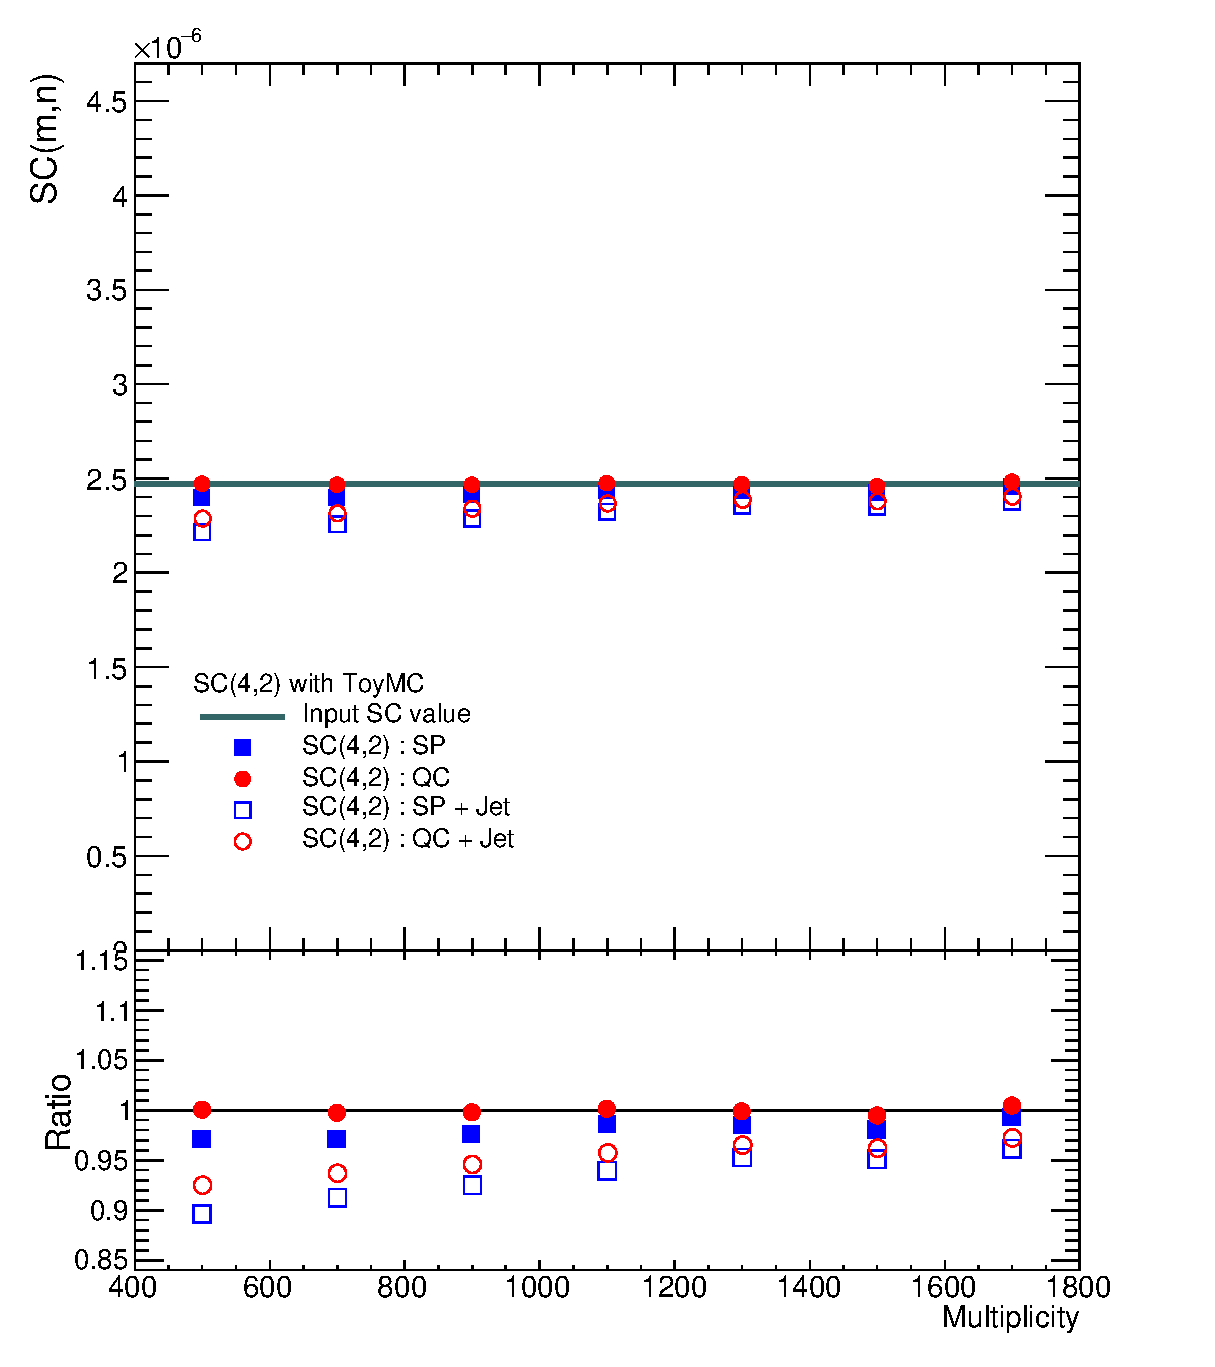
\includegraphics[width=9.0cm]{figures/figs_ToyMC/SC_Comparison_SC42_highmulti_ToyMC}}
\caption{The ToyMC results of SC(3,2) (left) and SC(4,2) (right) from 400 to 1800 multiplicity. The input values are drawn as green line. Closed markers are the results with SP and QC results without jet implementation(as same as previous results) and open markers are the results after PYHTHIA jet embedding. The ratio to the input values are drawn in bottom pad}
\label{fig:ToyMC_withJet}
\end{figure}


